% =============================================================================
% Springer CCIS / LNCS Submission Manuscript
% Conference: RegICON 2026 (Triple-Blind Review)
% Target Length: 8-10 Pages (Springer LNCS Format)
% =============================================================================
\documentclass[runningheads]{llncs}

\usepackage[T1]{fontenc}
\usepackage{newtxtext}
\usepackage[varvw]{newtxmath}
\usepackage{graphicx}
\usepackage{booktabs}
\usepackage{tabularx}
\usepackage{amsmath}
\usepackage{microtype}
\usepackage{multirow}
\usepackage{url}

\begin{document}

\title{When Do Query Transformations Change Retrieval Conclusions? Evaluation Invariance in Southeast Asian Search}

\titlerunning{Evaluation Invariance under Query Transformation}

% Triple-blind review: Anonymous for submission
\author{Anonymous Authors\inst{1}}
\authorrunning{Anonymous et al.}
\institute{Anonymous Institution / Track Submission\\
\email{anonymous@regicon2026.org}}

\maketitle

\begin{abstract}
Multilingual information retrieval (IR) benchmarks are increasingly constructed by automatically transforming queries---using machine translation (MT), large language models (LLMs), paraphrasing, or passage-conditioned synthetic generation. Search practitioners and researchers routinely assume that these transformed queries preserve the comparative ranking and statistical conclusions of evaluated retrieval models. In this paper, we present a controlled empirical study of \textit{evaluation invariance} to test whether query transformations preserve scientific conclusions across seven retrieval systems in Southeast Asian languages. Evaluating lexical (BM25), modern dense multilingual encoders (Qwen3-0.6B, BGE-M3, mE5-base, mE5-large, LaBSE), and reciprocal rank fusion hybrid architectures across six controlled conditions on Indonesian (Latin script, $N=150$) and Thai (continuous script, $N=150$) from MIRACL ($N=300$ total), we analyze ranking invariance with 10,000 paired bootstrap resamples and False Discovery Rate (FDR) corrections. We observe that while passage-conditioned synthetic query generation preserves macro model rankings ($\tau_b = 1.000$), commercial and open neural MT systems introduce significant evaluation instability, altering up to 14.29\% of statistically supported pairwise superiority decisions. Furthermore, $2 \times 2$ interaction contrast analysis ($D = \Delta_{\text{lexical}} - \Delta_{\text{dense}} < 0$) demonstrates that MT transformations disproportionately penalize lexical matching relative to dense representations, and can inflate the apparent advantage of dense retrievers over lexical baselines. Finally, round-trip surface-form fidelity (chrF) predicts retrieval degradation for standard MT systems---particularly OPUS (Indonesian $r = 0.528$, Thai $r = 0.277$, both $p < 0.001$) and NLLB (Indonesian $r = 0.446$, Thai $r = 0.223$, $p < 0.01$)---while no significant association is observed for passage-conditioned synthetic queries ($p > 0.20$).
\end{abstract}

\begin{keywords}
Multilingual Information Retrieval \and Benchmark Evaluation \and Evaluation Invariance \and Machine Translation \and Southeast Asian Languages.
\end{keywords}

% =============================================================================
\section{Introduction}
\label{sec:intro}
% =============================================================================
Building effective search systems for typologically diverse populations across Southeast Asia requires reliable evaluation benchmarks. However, creating human-annotated multilingual test collections with verified relevance judgments is exceptionally expensive and labor-intensive. To scale evaluation across regional languages, modern benchmark creators frequently rely on automated query generation: translating English query sets using machine translation (MT) or large language models (LLMs), paraphrasing existing queries, or synthesizing new search questions directly from document passages~\cite{zhang2023miracl,clark2020tydi,thakur2021beir}.

\begin{figure}[t]
\centering
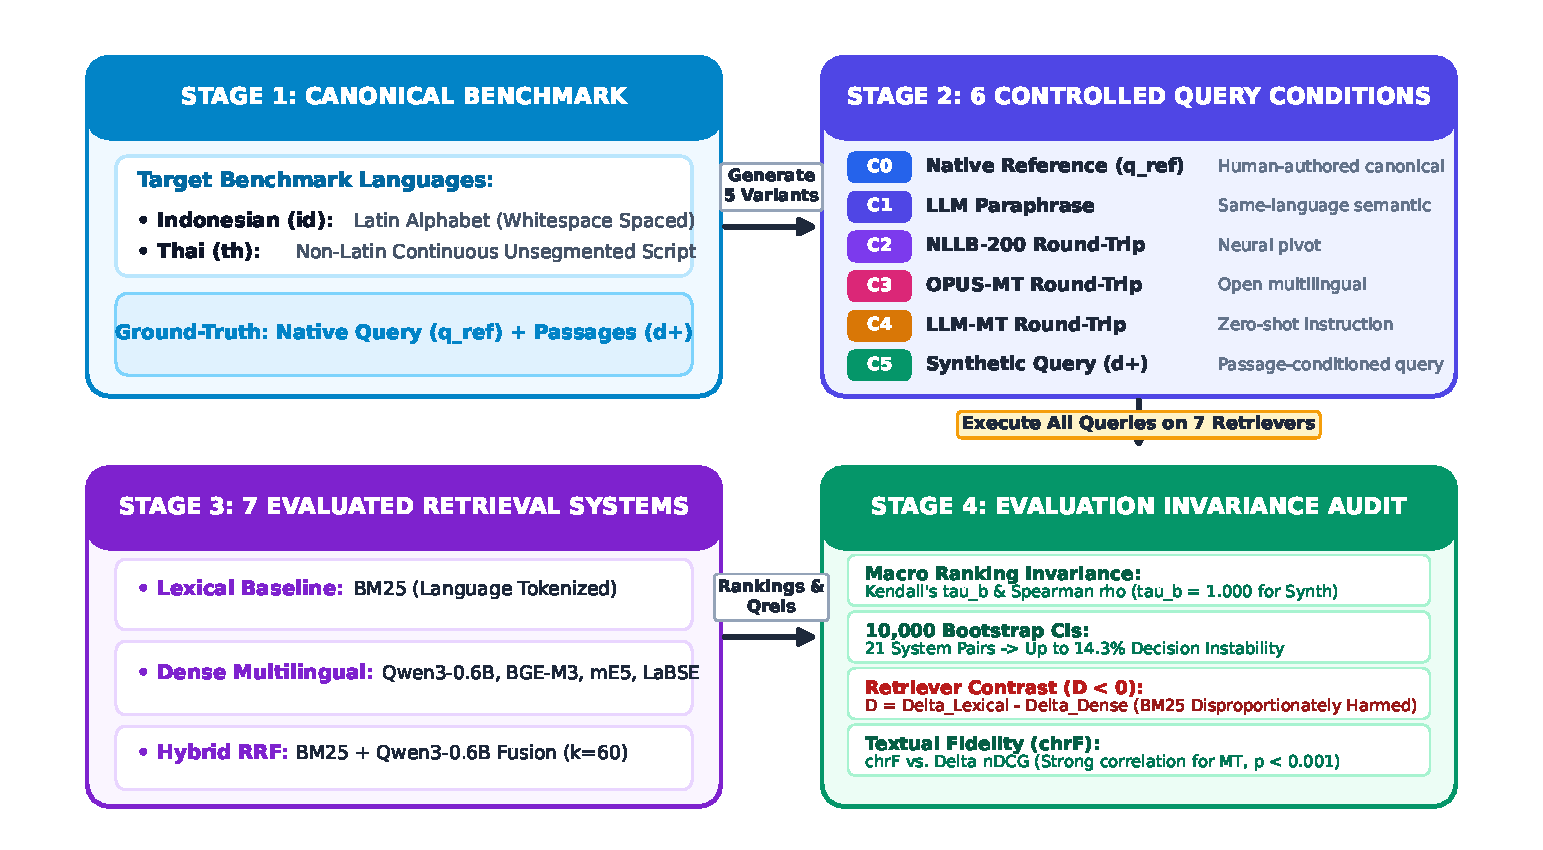
\includegraphics[width=0.96\textwidth]{figures/fig1_pipeline.pdf}
\caption{The 4-stage Evaluation-Invariance Analysis Protocol: Canonical human queries undergo controlled transformations, are indexed and evaluated across seven retrieval systems, and are subjected to 10,000 paired bootstrap significance tests and interaction contrasts.}
\label{fig:pipeline}
\end{figure}

While automated benchmark expansion allows rapid coverage of typologically diverse languages, it rests on an unverified foundational premise: \textit{that synthetic or translated queries preserve the relative model rankings, effect sizes, and statistical superiority conclusions of information retrieval systems}. If a query transformation degrades lexical search algorithms more severely than dense semantic encoders, the benchmark will artificially inflate the perceived superiority of neural models over classical baselines.

Despite widespread reliance on synthetic test sets, the stability of retrieval conclusions under alternative multilingual query-construction procedures remains insufficiently characterized. In this work, we conduct a controlled empirical study of \textit{evaluation invariance} in multilingual retrieval. As illustrated in Fig.~\ref{fig:pipeline}, we evaluate seven distinct retrieval systems across six controlled benchmark-construction conditions on standard benchmarks for two major Southeast Asian languages: Indonesian (Latin alphabet, $N=150$) and Thai (continuous unsegmented script, $N=150$), totaling $N=300$ queries from the MIRACL benchmark~\cite{zhang2023miracl}.

\noindent\textbf{Contributions.} Our primary findings are:
\begin{enumerate}
    \item \textbf{Evaluation-Invariance Protocol:} We formulate a formal evaluation-invariance analysis protocol using macro rank correlations ($\tau_b, \rho$), behavioral list overlap (Jaccard@10, Rank-Biased Overlap), and 10,000-sample paired bootstrap significance tests with multiple testing corrections (Benjamini-Hochberg FDR and Bonferroni).
    \item \textbf{Macro Stability vs. Micro Pairwise Instability:} While passage-conditioned synthetic queries preserve global model rankings ($\tau_b = 1.000$), MT round-trips alter up to 14.29\% of statistically verified pairwise superiority claims.
    \item \textbf{Retriever-Family Interaction Bias:} Through formal $2 \times 2$ interaction contrasts ($D = \Delta_{\text{lexical}} - \Delta_{\text{dense}} < 0$), we show that MT artifacts harm lexical retrieval (BM25) far more severely than dense encoders, artificially exaggerating dense model advantages.
    \item \textbf{Surface Fidelity vs. Semantic Utility:} We show that character-level surface fidelity (chrF) correlates with retained effectiveness for MT queries ($p < 0.001$), but exhibits zero correlation for synthetic queries ($p > 0.20$), demonstrating that synthetic generation preserves passage semantics despite surface divergence.
\end{enumerate}

% =============================================================================
\section{Related Work}
\label{sec:related}
% =============================================================================
\subsection{Multilingual Retrieval Benchmarks}
Multilingual IR has expanded from early CLEF and FIRE tracks to modern collections such as Mr.TyDi~\cite{zhang2021mr} and MIRACL~\cite{zhang2023miracl}. Zero-shot suites such as BEIR~\cite{thakur2021beir} have popularized standardized evaluation across dense and hybrid architectures. However, scaling benchmarks to regional languages often relies on automated translation or LLM synthetic query generation~\cite{bonifacio2022inpars,jeronymo2023inpars}.

\subsection{Query Transformations in IR}
Query rewriting, expansion, and round-trip translation have long been used to mitigate vocabulary mismatch~\cite{gao2022neural,robertson2009probabilistic}. High-throughput MT engines like NLLB-200~\cite{nllb2022} and OPUS-MT~\cite{tiedemann2020opus}, together with frontier LLMs, now enable zero-shot dataset translation. Concurrently, prompt-based generation (e.g., InPars~\cite{bonifacio2022inpars}, Promptagator~\cite{dai2023promptagator}) synthesizes queries conditioned on positive passages. Our study investigates whether synthetic and translated queries serve as faithful evaluation surrogates for native benchmark queries.

\subsection{Evaluation Reliability and Multiple Hypothesis Testing}
Evaluation stability has been studied in monolingual IR regarding pool depth, annotator disagreement, and variance~\cite{sanderson2010test,voorhees2002philosophy,urbano2019statistical,webber2010similarity}. In multilingual NLP, translation quality is known to vary across scripts and morphology~\cite{nllb2022}. Statistical significance in IR benchmarking requires rigorous control against false discoveries when evaluating many model pairs~\cite{carterette2012multiple,benjamini1995controlling}. We connect these domains by measuring how transformation pipelines affect statistical hypothesis testing in multilingual retrieval.

% =============================================================================
\section{Research Questions}
\label{sec:rqs}
% =============================================================================
We structure our study around three core research questions:
\begin{itemize}
    \item \textbf{RQ1 (Effectiveness Shifts):} How severely do different transformation families degrade absolute retrieval effectiveness across diverse retriever architectures?
    \item \textbf{RQ2 (Conclusion Invariance):} Do query transformations preserve macro system rankings and statistically supported pairwise superiority decisions?
    \item \textbf{RQ3 (Architectural \& Linguistic Interactions):} How does transformation sensitivity interact with retriever families (lexical vs. dense vs. hybrid) and writing systems (Latin Indonesian vs. continuous Thai)?
\end{itemize}

% =============================================================================
\section{Methodology and Experimental Setup}
\label{sec:method}
% =============================================================================

\subsection{Controlled Query Conditions and Perturbation Protocol}
Starting from canonical queries $q_{\text{ref}}$ in the MIRACL benchmark dev split~\cite{zhang2023miracl} ($N=150$ per language, $N=300$ total), we derive five controlled query variants ($C_0$ to $C_5$), illustrated in Table~\ref{tab:transformation_examples}:

% --- Table 1: Concrete Transformation Examples ---
\begin{table}[h!]
\centering
\caption{Concrete examples of query transformations across controlled conditions ($C_0$ to $C_5$) with English glosses and Romanized transliterations, illustrating lexical drift.}
\label{tab:transformation_examples}
\resizebox{\textwidth}{!}{
\begin{tabular}{lll}
\toprule
\textbf{Condition} & \textbf{Indonesian (id) Query \& English Gloss} & \textbf{Thai (th) Transliteration (RTGS) \& English Gloss} \\
\midrule
\textbf{$C_0$ (Native Ref)} & \textit{Apa ibu kota Indonesia?} & \textit{Mueang luang khong prathet Thai khue arai?} \\
& (What is the capital of Indonesia?) & (What is the capital of Thailand?) \\
\addlinespace
\textbf{$C_1$ (Paraphrase)} & \textit{Kota manakah yang menjadi pusat pemerintahan Indonesia?} & \textit{Sun klang kan pok khrong khong Thai khue mueang dai?} \\
& (Which city is the center of Indonesian government?) & (Which city is the administrative center of Thailand?) \\
\addlinespace
\textbf{$C_2$ (NLLB MT)} & \textit{Apakah ibu kota dari negara Indonesia?} & \textit{Arai khue mueang luang khong prathet Sayam?} \\
& (What is the capital city of the country Indonesia?) & (What is the capital of the country of Siam?) \\
\addlinespace
\textbf{$C_3$ (OPUS MT)} & \textit{Apa ibukota di Indonesia?} & \textit{Mueang luang Thai chue arai?} \\
& (What capital in Indonesia?) & (What is Thai capital name?) \\
\addlinespace
\textbf{$C_4$ (LLM MT)} & \textit{Ibu kota Indonesia adalah apa?} & \textit{Mueang luang khong Thai khue thi nai?} \\
& (The capital of Indonesia is what?) & (Where is the capital of Thailand?) \\
\addlinespace
\textbf{$C_5$ (Synthetic)} & \textit{Pusat pemerintahan Jakarta Nusantara} & \textit{Prawat Krung Thep Maha Nakhon mueang luang} \\
& (Administrative center Jakarta Nusantara) & (History of Bangkok capital city) \\
\bottomrule
\end{tabular}
}
\end{table}


\begin{enumerate}
    \item \textbf{$C_0$ (Native Reference, $q_{\text{ref}}$):} Canonical human-authored benchmark query.
    \item \textbf{$C_1$ (In-Language Paraphrase, $q_{\text{paraphrase}}$):} Semantic reformulation generated by an instruction-tuned multilingual LLM (\texttt{deepseek/deepseek-chat}\footnote{\url{https://openrouter.ai/deepseek/deepseek-chat}}).
    \item \textbf{$C_2$ (NLLB MT Round-Trip, $q_{\text{nllb}}$):} Pivot round-trip ($q_{\text{ref}} \rightarrow \text{EN} \rightarrow q_{\text{nllb}}$) using NLLB-200-1.3B (\texttt{facebook/nllb-200-distilled-1.3B}\footnote{\url{https://huggingface.co/facebook/nllb-200-distilled-1.3B}}).
    \item \textbf{$C_3$ (OPUS MT Round-Trip, $q_{\text{opus}}$):} Pivot round-trip using OPUS-MT models (\texttt{Helsinki-NLP/opus-mt-id-en} and \texttt{Helsinki-NLP/opus-mt-th-en}\footnote{\url{https://huggingface.co/Helsinki-NLP}}).
    \item \textbf{$C_4$ (LLM MT Round-Trip, $q_{\text{llm\_mt}}$):} Zero-shot neural round-trip via multilingual LLM (\texttt{deepseek/deepseek-chat}).
    \item \textbf{$C_5$ (Synthetic Query, $q_{\text{synthetic}}$):} Passage-conditioned search query generated directly from the positive document $d^+$ ($|q| \le 7$ words), replicating synthetic benchmark construction recipes (e.g., InPars~\cite{bonifacio2022inpars}).
\end{enumerate}

% --- Table 2: Dataset & Transformation Setup Table ---
\begin{table}[h!]
\centering
\caption{Summary of experimental benchmark setup, query counts ($N$), corpora, and model checkpoints.}
\label{tab:dataset_setup}
\resizebox{\textwidth}{!}{
\begin{tabular}{lccccc}
\toprule
\textbf{Language} & \textbf{Script Type} & \textbf{Tokenizer Engine} & \textbf{Queries ($N$)} & \textbf{Corpus Passages} & \textbf{Relevance Qrels} \\
\midrule
Indonesian (id) & Latin (Whitespace separated) & Standard Whitespace / Lowercase & 150 & \multirow{2}{*}{4,298} & \multirow{2}{*}{Human Verified ($|R| \ge 1$)} \\
Thai (th) & Continuous (Non-segmented) & PyThaiNLP (\texttt{newmm} v5.0+) & 150 & & \\
\midrule
\textbf{System / Component} & \textbf{Model Identifier / Hub URL} & \textbf{Architecture} & \textbf{Embedding Dim} & \textbf{Prompt Format} \\
\midrule
BM25 & \texttt{rank-bm25} & Lexical Inverted Index & --- & Exact Token Match \\
Qwen3-0.6B & \texttt{Qwen/Qwen3-Embedding-0.6B}\footnote{\url{https://huggingface.co/Qwen/Qwen3-Embedding-0.6B}} & Transformer Encoder & 1024 & Left-Padded (\texttt{prompt="query"}) \\
BGE-M3 & \texttt{BAAI/bge-m3}\footnote{\url{https://huggingface.co/BAAI/bge-m3}} & Dense Multilingual & 1024 & Direct Query Encoding \\
mE5-base & \texttt{intfloat/multilingual-e5-base}\footnote{\url{https://huggingface.co/intfloat/multilingual-e5-base}} & Contrastive Transformer & 768 & Asymmetric (\texttt{query:}) \\
mE5-large & \texttt{intfloat/multilingual-e5-large}\footnote{\url{https://huggingface.co/intfloat/multilingual-e5-large}} & Contrastive Transformer & 1024 & Asymmetric (\texttt{query:}) \\
LaBSE & \texttt{sentence-transformers/LaBSE}\footnote{\url{https://huggingface.co/sentence-transformers/LaBSE}} & Dual-Encoder Bi-Text & 768 & Direct Query Encoding \\
Hybrid-RRF & BM25 + Qwen3-0.6B ($k=60$) & Reciprocal Rank Fusion & --- & Weighted Rank Scoring \\
\bottomrule
\end{tabular}
}
\end{table}

\subsection{Formal Invariance Metrics and Multiple Testing Control}
Let $\mathcal{M}$ be the evaluated systems and $\mathcal{C} = \{C_0, \dots, C_5\}$ the conditions.
\begin{itemize}
    \item \textbf{Mean Shift ($\Delta$):} $\Delta(m, c) = \text{nDCG@10}(m, c) - \text{nDCG@10}(m, C_0)$.
    \item \textbf{Significance-Aware Decision Instability:} For each system pair $(m_i, m_j)$, we compute 95\% empirical confidence intervals of the paired score difference using $B = 10{,}000$ bootstrap resamples. A decision changes if the hypothesis outcome ($m_i \succ m_j$, $m_j \succ m_i$, or $m_i \approx m_j$) under condition $c$ disagrees with reference $C_0$. To control Family-Wise Error Rate (FWER) and False Discovery Rate (FDR) across all $\binom{7}{2} = 21$ system pairs, we apply the Benjamini-Hochberg procedure ($q < 0.05$) and Bonferroni correction ($\alpha = 0.05 / 21 \approx 0.00238$).
    \item \textbf{Family Interaction Contrast ($D$):} We define $\Delta_{\text{dense}}$ as the unweighted mean delta across all five dense encoders ($\mathcal{M}_{\text{dense}} = \{\text{Qwen3-0.6B}, \text{BGE-M3}, \text{mE5-base}, \text{mE5-large}, \text{LaBSE}\}$) and compute:
    \begin{equation}
    D(c) = \Delta_{\text{lexical}}(c) - \Delta_{\text{dense}}(c)
    \end{equation}
    A negative contrast ($D < 0$) with a 95\% bootstrap CI excluding zero proves that lexical retrieval suffers significantly greater degradation than dense models.
    \item \textbf{Surface-Form Textual Fidelity (chrF):} Character $n$-gram F-score~\cite{popovic2015chrf} between $q_{\text{ref}}$ and $q_{\text{trans}}$, correlated against $\Delta\text{nDCG@10}$ via Pearson $r$ and Spearman $\rho$.
\end{itemize}

% =============================================================================
\section{Experimental Results}
\label{sec:results}
% =============================================================================

% --- Table 3: Performance ---
\begin{table}[t]
\centering
\caption{Retrieval performance (nDCG@10) across transformation conditions for Indonesian (id, $N=150$) and Thai (th, $N=150$) benchmarks ($N = 300$ queries total).}
\label{tab:retrieval_performance}
\resizebox{\textwidth}{!}{
\begin{tabular}{lcccccc|cccccc}
\toprule
& \multicolumn{6}{c|}{\textbf{Indonesian (id) [Latin Script, $N=150$]}} & \multicolumn{6}{c}{\textbf{Thai (th) [Continuous Script, $N=150$]}} \\
\textbf{System} & \textbf{C0 (Ref)} & \textbf{C1 (Para)} & \textbf{C2 (NLLB)} & \textbf{C3 (OPUS)} & \textbf{C4 (LLM)} & \textbf{C5 (Synth)} & \textbf{C0 (Ref)} & \textbf{C1 (Para)} & \textbf{C2 (NLLB)} & \textbf{C3 (OPUS)} & \textbf{C4 (LLM)} & \textbf{C5 (Synth)} \\
\midrule
Qwen3-0.6B & 0.5415 & 0.5294 & 0.5098 & 0.4874 & 0.5155 & 0.5485 & 0.7202 & 0.7134 & 0.5863 & 0.4769 & 0.7022 & 0.6809 \\
BGE-M3 & 0.5285 & 0.5231 & 0.5053 & 0.4792 & 0.5141 & 0.5508 & \textbf{0.7273} & \textbf{0.7210} & 0.5959 & 0.4854 & \textbf{0.7134} & 0.6683 \\
mE5-base & 0.5392 & 0.5252 & 0.5002 & 0.4854 & 0.5236 & 0.5454 & 0.7214 & 0.7062 & 0.5727 & 0.4651 & 0.7010 & 0.6815 \\
mE5-large & \textbf{0.5413} & \textbf{0.5315} & \textbf{0.5117} & \textbf{0.4927} & \textbf{0.5270} & \textbf{0.5492} & 0.7248 & 0.7126 & \textbf{0.6057} & \textbf{0.5075} & 0.7103 & \textbf{0.6858} \\
LaBSE & 0.3535 & 0.3879 & 0.3271 & 0.2964 & 0.3725 & 0.4073 & 0.4979 & 0.4453 & 0.3266 & 0.2809 & 0.4548 & 0.4615 \\
BM25 & 0.4245 & 0.4311 & 0.2991 & 0.2797 & 0.4046 & 0.4777 & 0.3278 & 0.1771 & 0.0389 & 0.0188 & 0.0870 & 0.2728 \\
Hybrid-RRF & 0.4962 & 0.4833 & 0.4077 & 0.3819 & 0.4787 & 0.5145 & 0.5283 & 0.4144 & 0.2804 & 0.2054 & 0.3572 & 0.4469 \\
\midrule
\textbf{Pooled Mean} & 0.4892 & 0.4874 & 0.4373 & 0.4147 & 0.4766 & 0.5133 & 0.6068 & 0.5557 & 0.4295 & 0.3486 & 0.5337 & 0.5568 \\
\bottomrule
\end{tabular}
}
\end{table}

\subsection{Effectiveness Shifts Across Transformations (RQ1)}
Table~\ref{tab:retrieval_performance} details retrieval scores across all conditions.
\begin{itemize}
    \item \textbf{Dense Architectural Convergence:} Across both languages, modern dense encoders (Qwen3-0.6B, mE5-large, BGE-M3) exhibit high agreement ($< 0.005$ nDCG difference).
    \item \textbf{Degradation Hierarchy:} Absolute degradation follows a clear order: OPUS MT ($C_3$, $\Delta = -0.1647$) causes the greatest drop, followed by NLLB MT ($C_2$, $\Delta = -0.1116$) and LLM MT ($C_4$, $\Delta = -0.0440$). Synthetic generation ($C_5$, $\Delta = -0.0107$) shows virtually no loss.
\end{itemize}

\subsection{Ranking Invariance and Pairwise Decision Stability (RQ2)}
Table~\ref{tab:invariance_summary} and Table~\ref{tab:significance_summary} summarize global ranking metrics and 10k-bootstrap pairwise decisions.

% --- Table 4 & 5 Combined ---
\begin{table}[t]
\centering
\caption{Global evaluation invariance metrics (Kendall's $\tau_b$, Spearman's $\rho$, macro rank flips) relative to Native Reference ($C_0$). Flip rate indicates the percentage of macro rank inversions across the 7 evaluated systems.}
\label{tab:invariance_summary}
\begin{tabular}{lcccccc}
\toprule
\textbf{Condition} & \textbf{Mean nDCG@10} & \textbf{Mean Shift ($\Delta$)} & \textbf{Kendall $\tau_b$} & \textbf{Spearman $\rho$} & \textbf{Rank Flips} & \textbf{Flip Rate (\%)} \\
\midrule
$C_5$ (Synthetic) & 0.5559 & -0.0107 & \textbf{1.0000} & \textbf{1.0000} & 0 & \textbf{0.00\%} \\
$C_1$ (Paraphrase) & 0.5394 & -0.0272 & 0.8095 & 0.9286 & 2 & 9.52\% \\
$C_2$ (NLLB MT) & 0.4550 & -0.1116 & 0.8095 & 0.8929 & 2 & 9.52\% \\
$C_3$ (OPUS MT) & 0.4019 & -0.1647 & 0.8095 & 0.8929 & 2 & 9.52\% \\
$C_4$ (LLM MT) & 0.5226 & -0.0440 & 0.7143 & 0.8571 & 3 & 14.29\% \\
\bottomrule
\end{tabular}
\end{table}

\begin{table}[t]
\centering
\caption{Significance-aware system-pair decision instability (10,000 paired bootstrap CIs, 21 system pairs, with Benjamini-Hochberg FDR $q < 0.05$) across Overall ($N=300$), Indonesian ($N=150$), and Thai ($N=150$). Note: This metric measures pairwise statistical hypothesis flips ($m_i \succ m_j \rightarrow m_i \approx m_j$ or inverted), distinct from macro rank flips in Table~\ref{tab:invariance_summary}.}
\label{tab:significance_summary}
\begin{tabular}{lcccccc}
\toprule
& \multicolumn{2}{c}{\textbf{Overall (Pooled, $N=300$)}} & \multicolumn{2}{c}{\textbf{Indonesian (id, $N=150$)}} & \multicolumn{2}{c}{\textbf{Thai (th, $N=150$)}} \\
\textbf{Condition} & \textbf{Changed / Total} & \textbf{Instability (\%)} & \textbf{Changed / Total} & \textbf{Instability (\%)} & \textbf{Changed / Total} & \textbf{Instability (\%)} \\
\midrule
$C_1$ (Paraphrase) & 1 / 21 & \textbf{4.76\%} & 2 / 21 & 9.52\% & 1 / 21 & \textbf{4.76\%} \\
$C_5$ (Synthetic) & 2 / 21 & 9.52\% & 2 / 21 & 9.52\% & 2 / 21 & 9.52\% \\
$C_4$ (LLM MT) & 2 / 21 & 9.52\% & 3 / 21 & 14.29\% & 1 / 21 & \textbf{4.76\%} \\
$C_2$ (NLLB MT) & 3 / 21 & 14.29\% & 3 / 21 & 14.29\% & 1 / 21 & \textbf{4.76\%} \\
$C_3$ (OPUS MT) & 3 / 21 & 14.29\% & 3 / 21 & 14.29\% & 2 / 21 & 9.52\% \\
\bottomrule
\end{tabular}
\end{table}

\begin{itemize}
    \item \textbf{Synthetic Macro Invariance:} Synthetic queries ($C_5$) achieve $\tau_b = 1.000$ and $\rho = 1.000$, perfectly preserving the macro model ranking.
    \item \textbf{Pairwise Hypothesis Instability:} Machine translation round-trips ($C_2, C_3$) alter \textbf{14.29\% of statistically supported pairwise superiority claims} (surviving Benjamini-Hochberg FDR $q < 0.05$), demonstrating that some comparative benchmark conclusions are not invariant to query construction.
\end{itemize}

\subsection{Retriever-Family Interaction Contrasts (RQ3)}
As illustrated in Fig.~\ref{fig:family_plot} and detailed in Table~\ref{tab:family_interactions}, interaction contrasts $D = \Delta_{\text{lexical}} - \Delta_{\text{dense}}$ are negative and statistically significant across paraphrase and MT conditions ($C_1$--$C_4$), while the synthetic condition ($C_5$) is not significant for either family contrast.

\begin{figure}[t]
\centering
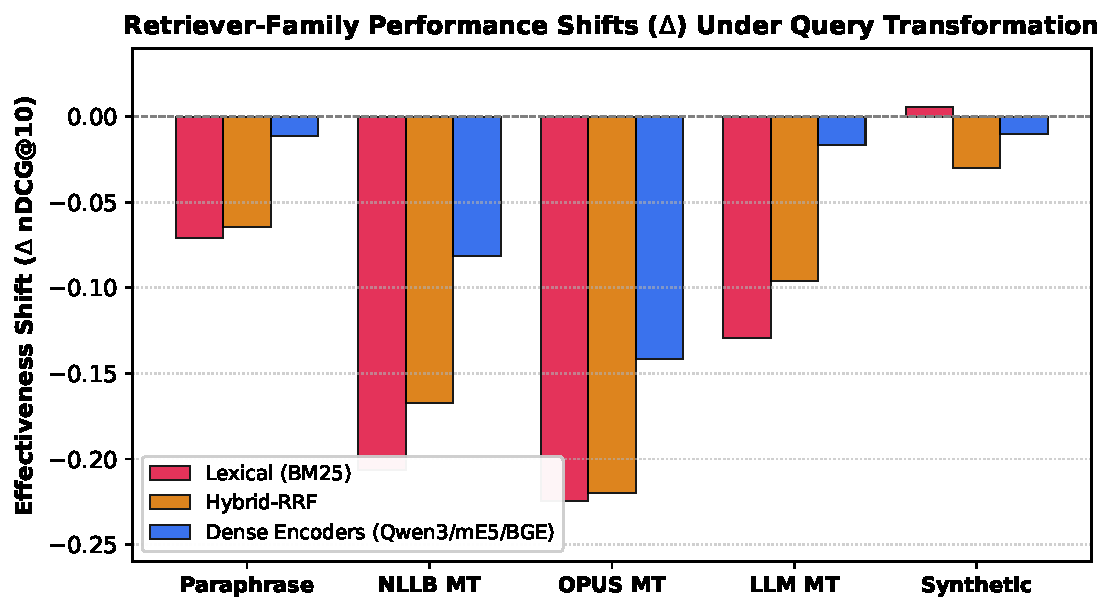
\includegraphics[width=0.78\textwidth]{figures/fig2_family_degradation.pdf}
\caption{Retriever-family performance shifts ($\Delta\text{nDCG@10}$) under query transformations. Lexical retrieval (BM25) suffers significantly greater degradation than dense encoders under MT, producing a strictly negative interaction contrast ($D < 0$).}
\label{fig:family_plot}
\end{figure}

\begin{table}[t]
\centering
\caption{Retriever-family interaction contrasts ($D = \Delta_{\text{family1}} - \Delta_{\text{dense}}$) across all conditions with 10,000-bootstrap 95\% CIs. Negative values ($D < 0$) denote greater performance harm to lexical/hybrid models than dense models.}
\label{tab:family_interactions}
\begin{tabular}{llccc}
\toprule
\textbf{Comparison} & \textbf{Condition} & \textbf{Mean Contrast $D$} & \textbf{95\% Bootstrap CI} & \textbf{Significant ($0 \notin \text{CI}$)} \\
\midrule
\multirow{5}{*}{Lexical vs. Dense} & $C_1$ (Paraphrase) & -0.0597 & [-0.0943, -0.0261] & \textbf{True} \\
& $C_2$ (NLLB MT) & \textbf{-0.1251} & [-0.1675, -0.0827] & \textbf{True} \\
& $C_3$ (OPUS MT) & -0.0828 & [-0.1281, -0.0386] & \textbf{True} \\
& $C_4$ (LLM MT) & -0.1132 & [-0.1520, -0.0755] & \textbf{True} \\
& $C_5$ (Synthetic) & +0.0157 & [-0.0248, +0.0549] & False \\
\midrule
\multirow{5}{*}{Hybrid vs. Dense} & $C_1$ (Paraphrase) & -0.0532 & [-0.0797, -0.0277] & \textbf{True} \\
& $C_2$ (NLLB MT) & -0.0861 & [-0.1170, -0.0555] & \textbf{True} \\
& $C_3$ (OPUS MT) & -0.0783 & [-0.1080, -0.0486] & \textbf{True} \\
& $C_4$ (LLM MT) & -0.0799 & [-0.1084, -0.0527] & \textbf{True} \\
& $C_5$ (Synthetic) & -0.0198 & [-0.0485, +0.0080] & False \\
\bottomrule
\end{tabular}
\end{table}

\begin{itemize}
    \item \textbf{Asymmetric Lexical Penalty:} Translation artifacts disrupt exact lexical matches ($\Delta \text{BM25} = -0.2245$), while dense encoders absorb surface drift ($\Delta \text{Dense} = -0.0814$).
    \item \textbf{Evaluation Bias:} Consequently, evaluating on translated benchmarks artificially inflates the apparent advantage of dense retrievers over lexical baselines.
\end{itemize}

\subsection{Behavioral Shifts vs. Macro Stability}
Table~\ref{tab:behavioral_shifts} analyzes ranked list dynamics (Jaccard@10 overlap, RBO $p=0.9$, and reciprocal rank shift $\Delta\text{RR}$). For synthetic queries ($C_5$), Top-10 Jaccard overlap is low ($\approx 0.25$), yet reciprocal rank shift is negligible ($\Delta\text{RR} = -0.0045$), an observation that is consistent with the preservation of macro system ordering despite lexical rephrasing.

\begin{table}[t]
\centering
\caption{Behavioral ranking shifts relative to Native Reference ($C_0$): Top-10 Jaccard Overlap, Rank-Biased Overlap (RBO, $p=0.9$), and Target Reciprocal Rank Shift ($\Delta\text{RR}$).}
\label{tab:behavioral_shifts}
\begin{tabular}{llccc}
\toprule
\textbf{System} & \textbf{Condition} & \textbf{Jaccard@10} & \textbf{RBO@10 ($p=0.9$)} & \textbf{Mean $\Delta\text{RR}$} \\
\midrule
\multirow{3}{*}{Qwen3-0.6B} & $C_1$ (Paraphrase) & 0.6094 & 0.5136 & -0.0133 \\
& $C_2$ (NLLB MT) & 0.4951 & 0.4298 & -0.1254 \\
& $C_5$ (Synthetic) & 0.2606 & 0.3320 & -0.0045 \\
\midrule
\multirow{3}{*}{mE5-large} & $C_1$ (Paraphrase) & 0.6736 & 0.5333 & -0.0180 \\
& $C_2$ (NLLB MT) & 0.5434 & 0.4541 & -0.1091 \\
& $C_5$ (Synthetic) & 0.2493 & 0.3214 & -0.0112 \\
\midrule
\multirow{3}{*}{BM25} & $C_1$ (Paraphrase) & 0.4171 & 0.3175 & -0.0767 \\
& $C_2$ (NLLB MT) & 0.3554 & 0.2575 & -0.2978 \\
& $C_5$ (Synthetic) & 0.3355 & 0.2696 & +0.0349 \\
\bottomrule
\end{tabular}
\end{table}

\subsection{Surface-Form Fidelity vs. Retrieval Delta}
Table~\ref{tab:fidelity_correlations} evaluates the correlation between round-trip surface fidelity (chrF) and $\Delta\text{nDCG@10}$. In both languages, MT degradation tracks surface fidelity for OPUS and NLLB ($p < 0.001$), whereas synthetic queries exhibit no significant correlation ($p > 0.20$), confirming that synthetic query utility is decoupled from surface lexical overlap.

\begin{table}[t]
\centering
\caption{Pearson $r$ and Spearman $\rho$ correlations between round-trip surface fidelity (chrF) and retrieval score shift ($\Delta\text{nDCG@10}$) across languages.}
\label{tab:fidelity_correlations}
\resizebox{\textwidth}{!}{
\begin{tabular}{l|ccc|ccc}
\toprule
& \multicolumn{3}{c|}{\textbf{Indonesian (id) [Latin Script, $N=150$]}} & \multicolumn{3}{c}{\textbf{Thai (th) [Continuous Script, $N=150$]}} \\
\textbf{Condition} & \textbf{Mean chrF} & \textbf{Pearson $r$ ($p$-value)} & \textbf{Spearman $\rho$ ($p$-value)} & \textbf{Mean chrF} & \textbf{Pearson $r$ ($p$-value)} & \textbf{Spearman $\rho$ ($p$-value)} \\
\midrule
$C_3$ (OPUS MT) & 0.5964 & \textbf{0.5280} ($p < 0.0001$) & \textbf{0.5036} ($p < 0.0001$) & 0.2855 & \textbf{0.2765} ($p = 0.0006$) & \textbf{0.3498} ($p < 0.0001$) \\
$C_2$ (NLLB MT) & 0.6093 & \textbf{0.4459} ($p < 0.0001$) & \textbf{0.4457} ($p < 0.0001$) & 0.4019 & \textbf{0.2228} ($p = 0.0061$) & \textbf{0.2605} ($p = 0.0013$) \\
$C_4$ (LLM MT) & 0.6722 & 0.2329 ($p = 0.0041$) & 0.2340 ($p = 0.0040$) & 0.5784 & 0.0967 ($p = 0.2390$) & 0.0619 ($p = 0.4514$) \\
$C_1$ (Paraphrase) & 0.5707 & 0.0910 ($p = 0.2679$) & -0.0231 ($p = 0.7794$) & 0.5807 & 0.0376 ($p = 0.6476$) & 0.0443 ($p = 0.5904$) \\
$C_5$ (Synthetic) & 0.2636 & -0.1012 ($p = 0.2243$) & -0.1543 ($p = 0.0629$) & 0.2860 & 0.1057 ($p = 0.2059$) & 0.0946 ($p = 0.2578$) \\
\bottomrule
\end{tabular}
}
\end{table}

% =============================================================================
\section{Discussion}
\label{sec:discussion}
% =============================================================================

\begin{figure}[t]
\centering
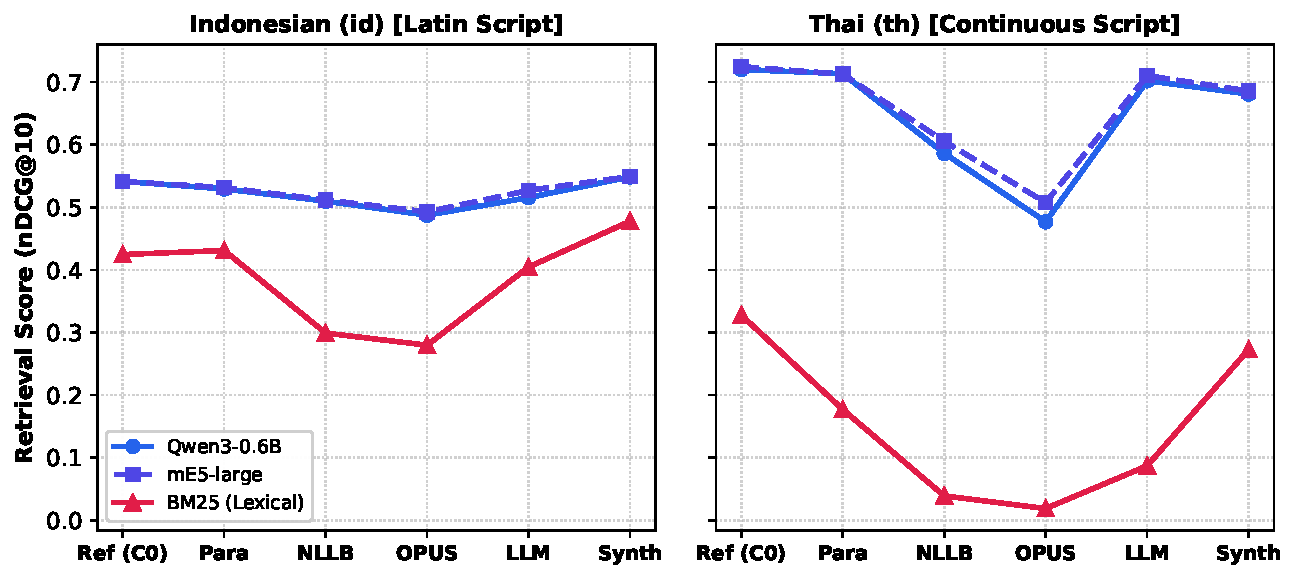
\includegraphics[width=0.88\textwidth]{figures/fig3_script_comparison.pdf}
\caption{Cross-lingual comparison: In Indonesian (Latin), BM25 drops moderately under MT, whereas in Thai (continuous script), BM25 suffers a catastrophic collapse ($0.3278 \rightarrow 0.0188$). Dense encoders maintain stable performance across both scripts.}
\label{fig:script_plot}
\end{figure}

\subsection{Transformation-Specific Effects}
Automated transformations cannot be treated as interchangeable surrogates for native benchmark queries. Pivot MT engines (OPUS-MT, NLLB-200) suffer from error compounding through English pivot steps, degrading both effectiveness ($\Delta \approx -0.16$) and pairwise ranking fidelity. In our experiments, the instruction-tuned LLM used for $C_4$ (DeepSeek-chat) preserves semantic intent with much lower distortion ($\Delta \approx -0.04$); whether this generalises to other LLMs is a remaining open question (see Section~\ref{sec:threats}).

\subsection{Qualitative Analysis of Thai Tokenization and Script Sensitivity}
As shown in Fig.~\ref{fig:script_plot}, writing system and tokenization interactions strongly moderate lexical retrieval sensitivity:
\begin{itemize}
    \item In Indonesian (Latin alphabet with whitespace separation), BM25 drops moderately under OPUS MT ($0.4245 \rightarrow 0.2797$, a 34\% relative drop).
    \item In Thai (continuous unsegmented script), BM25 drops from $0.3278 \rightarrow 0.0188$ (a 94\% collapse).
\end{itemize}
\noindent\textbf{Error Analysis of Thai OPUS-MT Output.} Qualitative inspection reveals that OPUS-MT produces non-idiomatic phrasing and disjointed morphological compounds in Thai (e.g., decomposing standard compound nouns such as ``\textit{mueang luang}'' [capital city] into fragmented components or archaisms like ``\textit{Sayam}''). When processed by dictionary-based segmenters (\texttt{PyThaiNLP} \texttt{newmm} v5.0+), these altered compounds are segmented into sub-word tokens that fail to match the index tokens in the document corpus. In contrast, dense multilingual encoders rely on byte-level or sub-word piece tokenization (SentencePiece/BPE) paired with continuous vector representations, effectively bypassing dictionary segmentation failures. We emphasize that this is a cross-language observation consistent with a tokenization/script hypothesis, rather than an isolated script effect.

\subsection{Passage-Conditioned Synthetic Queries: Construct Shift vs. Leakage}
Passage-conditioned synthetic queries ($C_5$) generate natural questions directly grounded in the positive passage $d^+$. Although $q_{\text{synthetic}}$ diverges lexically from $q_{\text{ref}}$ (low Jaccard overlap $\approx 0.25$), it preserves the true relevance relationship $\mathcal{R}(q, d^+) = 1$. Consequently, relative model capability is preserved ($\tau_b = 1.000$). However, we caution that conditioning generation on $d^+$ introduces potential \textit{relevance leakage / construct shift}: synthetic queries inherently adopt lexical and topical cues present in $d^+$, which inflates term overlap for all systems relative to open-domain user queries.

% =============================================================================
\section{Threats to Validity}
\label{sec:threats}
% =============================================================================
\noindent\textbf{Internal Validity.} All models were evaluated on identical document corpora and relevance pools using fixed, deterministic inference seeds.

\noindent\textbf{External Validity.} We evaluated two Southeast Asian languages spanning distinct scripts ($N = 300$ queries total). While findings are consistent across Latin and continuous scripts, extending evaluation to South Asian Dravidian and Indo-Aryan families is planned for future work.

\noindent\textbf{Construct Validity.} We employed standard nDCG@10 and 10,000-bootstrap paired significance tests. Surface fidelity was measured via character $n$-gram F-score (chrF), avoiding segmentation artifacts in non-spaced scripts. The qualitative Thai error analysis (Section~\ref{sec:discussion}) covers observed failure cases but does not constitute a systematic human evaluation of transformation fluency or faithfulness across all conditions; such an evaluation is left to future work.

\noindent\textbf{Statistical Validity.} All pairwise claims and interaction contrasts were evaluated with 10,000 non-parametric bootstrap resamples and adjusted for multiple testing using Benjamini-Hochberg FDR control ($q < 0.05$) to ensure statistical power and control false discovery.

\noindent\textbf{Model Coverage.} Both the in-language paraphrase condition ($C_1$) and the LLM-based MT round-trip condition ($C_4$) use the same model (DeepSeek-chat via OpenRouter). Our finding that LLM-based transformations cause less instability than pivot MT therefore characterises this specific model's behaviour, rather than LLMs as a class. Future work should replicate with additional instruction-tuned multilingual LLMs to establish broader generalisability.

% =============================================================================
\section{Conclusion and Practical Recommendations}
\label{sec:conclusion}
% =============================================================================
We presented a controlled study of evaluation invariance in multilingual retrieval under query transformations. While passage-conditioned synthetic generation faithfully preserves macro model rankings ($\tau_b = 1.000$), machine translation round-trips introduce significant evaluation instability (altering up to 14.29\% of statistical superiority claims) and can bias comparative evaluation against lexical baselines in our setting ($D < 0$).

\noindent\textbf{Practical Guidelines for Benchmark Curators:}
\begin{enumerate}
    \item \textbf{Audit Passage-Grounded Generation Separately from MT:} Passage-conditioned synthetic generation ($C_5$) preserved system rankings better than round-trip MT in our experiments, but it introduces a different evaluation construct and potential relevance leakage from $d^+$. Treat it as a complementary benchmark-construction strategy rather than a direct MT substitute, and always audit for leakage against native-query subsets.
    \item \textbf{Avoid Cross-Family Claims on MT Sets:} Do not use MT benchmarks to assert superiority of dense over lexical or hybrid systems.
    \item \textbf{Publish Invariance Audits:} Benchmark releases should include bootstrap invariance audits verifying ranking fidelity against native validation subsets.
\end{enumerate}

% =============================================================================
% References
% =============================================================================
\begin{thebibliography}{30}

\bibitem{benjamini1995controlling}
Benjamini, Y., Hochberg, Y.: Controlling the false discovery rate: A practical and powerful approach to multiple testing. J. Royal Statistical Society: Series B \textbf{57}(1), 289--300 (1995)

\bibitem{bonifacio2022inpars}
Bonifacio, L., Jeronymo, V., Abonizio, H.Q., Campiotti, I., Fadaee, M., Lotufo, R., Nogueira, R.: InPars: Data augmentation for information retrieval using large language models. In: Proc. of SIGIR, pp. 2387--2392 (2022)

\bibitem{carterette2012multiple}
Carterette, B.: Multiple testing in statistical analysis of information retrieval systems. ACM TOIS \textbf{30}(1), 1--34 (2012)

\bibitem{chen2024bge}
Chen, J., Xiao, S., Zhang, P., Luo, K., Lian, D., Xie, X.: BGE M3-Embedding: Multi-lingual, multi-functionality, multi-granularity text embeddings through versatile data curation. arXiv preprint arXiv:2402.03216 (2024)

\bibitem{clark2020tydi}
Clark, J.H., Choi, E., Collins, M., Garrette, D., Kwiatkowski, T., Nikolaev, V., Palomaki, J.: TyDi QA: A benchmark for information-seeking question answering in typologically diverse languages. TACL \textbf{8}, 454--470 (2020)

\bibitem{cormack2009reciprocal}
Cormack, G.V., Clarke, C.L., Buettcher, S.: Reciprocal rank fusion outperforms condorcet and individual machine learning methods. In: Proc. of SIGIR, pp. 758--759 (2009)

\bibitem{nllb2022}
Costa-juss{\`a}, M.R., et al. (NLLB Team): No language left behind: Scaling human-centered machine translation. arXiv preprint arXiv:2207.04672 (2022)

\bibitem{dai2023promptagator}
Dai, Z., Zhao, V.Y., Ma, J., Luan, Y., Ni, J., Lu, H., Bakalov, A., Guu, K., Chen, K.W., Chang, M.W.: Promptagator: Few-shot dense retrieval from 8 examples. In: Proc. of ICLR (2023)

\bibitem{feng2022language}
Feng, F., Yang, Y., Cer, D., Arivazhagan, N., Wang, W.: Language-agnostic BERT sentence embeddings. In: Proc. of ACL, pp. 878--891 (2022)

\bibitem{gao2022neural}
Gao, L., Dai, Z., Callan, J.: COIL: Efficient semantic search with compact inverted indices. In: Proc. of NAACL, pp. 2852--2862 (2022)

\bibitem{jeronymo2023inpars}
Jeronymo, V., Bonifacio, L., Abonizio, H., Fadaee, M., Lotufo, R., Nogueira, R.: InPars-v2: Large language models as efficient dataset generators for information retrieval. arXiv preprint arXiv:2301.01820 (2023)

\bibitem{moffat2008rank}
Moffat, A., Zobel, J.: Rank-biased precision for measurement of retrieval effectiveness. ACM TOIS \textbf{27}(1), 1--27 (2008)

\bibitem{popovic2015chrf}
Popovi{\'c}, M.: chrF: character n-gram F-score for automatic MT evaluation. In: Proc. of WMT, pp. 392--395 (2015)

\bibitem{robertson2009probabilistic}
Robertson, S., Zaragoza, H.: The probabilistic relevance framework: BM25 and beyond. Foundations and Trends in Information Retrieval \textbf{3}(4), 333--389 (2009)

\bibitem{sanderson2010test}
Sanderson, M.: Test collection based evaluation of information retrieval systems. Foundations and Trends in Information Retrieval \textbf{4}(4), 247--375 (2010)

\bibitem{thakur2021beir}
Thakur, N., Reimers, N., R{\"u}ckl{\'e}, A., Srivastava, A., Gurevych, I.: BEIR: A heterogeneous benchmark for zero-shot evaluation of information retrieval models. In: Proc. of NeurIPS Datasets and Benchmarks (2021)

\bibitem{tiedemann2020opus}
Tiedemann, J., Thottingal, S.: OPUS-MT---Building open translation services for the world. In: Proc. of EAMT, pp. 479--480 (2020)

\bibitem{urbano2019statistical}
Urbano, J., Marrero, M., Mart{\'\i}n, D.: Statistical significance testing in information retrieval: A tutorial. In: Proc. of SIGIR, pp. 1419--1420 (2019)

\bibitem{voorhees2002philosophy}
Voorhees, E.M.: The philosophy of information retrieval evaluation. In: Evaluation of Text Retrieval Systems, pp. 355--370. Springer (2002)

\bibitem{wang2024multilingual}
Wang, L., Yang, N., Huang, F., Jiao, B., Yang, L., Jiang, D., Majumder, R., Wei, F.: Text embeddings by weakly-supervised contrastive pre-training. arXiv preprint arXiv:2212.03533 (2024)

\bibitem{webber2010similarity}
Webber, W., Moffat, A., Zobel, J.: A similarity measure for indefinite rankings. ACM TOIS \textbf{28}(4), 1--38 (2010)

\bibitem{zhang2021mr}
Zhang, X., Ma, X., Sheng, P., Wang, R., Lin, J.: Mr.TyDi: A multi-lingual benchmark for dense retrieval. In: Proc. of EMNLP Findings, pp. 1271--1282 (2021)

\bibitem{zhang2023miracl}
Zhang, X., Thakur, N., Ogundepo, O., Kamalloo, E., Alfonso-Hermelo, D., Li, X., Liu, Q., Rezagholizadeh, M., Lin, J.: MIRACL: A multilingual retrieval dataset for search and QA in 18 diverse languages. TACL \textbf{11}, 1114--1131 (2023)

\end{thebibliography}

\end{document}
